\section{Numerical Examples}

\subsection{Cholesky Factorization}

\begin{frame}{Cholesky Factorization}
	
	\begin{block}{Data}
		Exponential covariance matrix, $\boldsymbol{\Sigma}_{ij}=exp(-\lVert \mathbf{s}_i-\mathbf{s}_j \rVert/\beta)$ is set with $\beta=0.3$. $n$ points, $\mathbf{s}_1,\cdots,\mathbf{s}_n$ is evenly distributed over unique square with Morton's order which defined recursively as described in figure \ref{fig:morton}.
	\end{block}

	\begin{figure}[h]
		\centering
		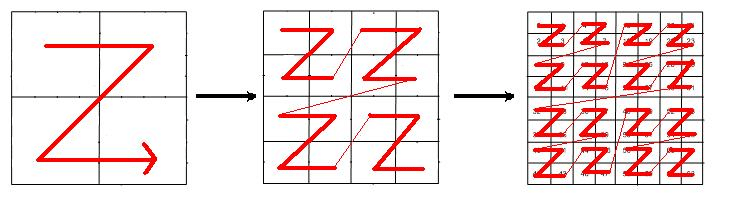
\includegraphics[width=.7\linewidth]{figs/Morton.jpg}
		\caption{Morton's order \citep{salem2016comparative}}
		\label{fig:morton}
	\end{figure}
\end{frame}

\begin{frame}{Cholesky Factorization}
	\begin{block}{Methods}
		\begin{enumerate}
			\item The \textit{chol} function from \textbf{LinearAlgebra} package
			\item The \textit{dpotrf} from \textbf{LAPACK} package
			\item Hierarchical cholesky decomposition which suggested by \citet{hackbusch2015hierarchical} are implemented. 
		\end{enumerate}
	\end{block}
	
	\begin{itemize}
		\item With various $n$, three Cholesky methods are applied and results are below table \ref{tab:table1}. 
		\item In low rank approximation at algorithm \ref{alg:hchol}, rank is about $n^{1/4}$.
		\item Hierarchical cholesky decomposition provides $\boldsymbol{\Sigma}\approx L_HL_H^T$. 
		\item Its relative error is defined as 
		$\dfrac{\lVert\boldsymbol{\Sigma}-L_HL_H^T\rVert_2}{\lVert\boldsymbol{\Sigma}\rVert_2}$
	\end{itemize}
	
\end{frame}

\begin{frame}{Cholesky Factorization}

\begin{table}[h]
	\centering
	\resizebox{.8\textwidth}{!}{
		\begin{tabular}{@{}ccccc@{}}
			\toprule
			n & 256 & 1024 & 4096 & 16384 \\ \midrule
			chol & 0.001s & 0.0097s & 0.414s & 156.3s \\
			dpotrf & 0.0007s & 0.0132s & 0.431s & 154.1s \\
			hierarchical cholesky & 0.153s & 0.076s & 0.916s & 37.3s \\
			Error of hierarchical cholesky & 1.06e-7 & 9.97e-7 & 1.11e-3 & 1.87e-3 \\  \bottomrule
		\end{tabular}%
	}
	\caption{Excution times for Cholesky factorization}
	\label{tab:table1}
\end{table}

\begin{block}{Results}
	\begin{itemize}
		\item Hierarchical cholesky decomposition is more efficient than other classical cholesky method with large dimension.
		\item Table \ref{tab:table1} ensures accuracy of hierarchical cholesky decomposition proposed by \citet{hackbusch2015hierarchical}.
	\end{itemize}
\end{block}

\end{frame}

\subsection{Multidimensional Conditioning Approximations}

\begin{frame}{Multivariate Normal Probabilities} 

	\begin{block}{Methods}
		\begin{enumerate}
			\item Classical Monte Carlo(MC) is estimate probabilities from acceptance ratio
			\item Richtmyer Quasi-Monte Carlo(QMC) introduced in subsection \ref{subsec:qmc}
		\end{enumerate}
	\end{block}

	\begin{block}{Settings}
		\begin{itemize}
			% \item We implement \texttt{mvn}, the function that calculate multivariate normal probabilities using Richtmyer QMC method introduced in subsection \ref{subsec:qmc}. 
			\item Varying sample size $N$ and dimension $d$, two Monte Carlo methods are compared and results are below table \ref{tab:results_mc} and \ref{tab:results_qmc}. 
			\item Set $\Sigma = I_d$, $\mathbf{a}_i = -\infty$ and $\mathbf{b}_i = 0$, i.e. true probabilities are $1/2^d$s
			\item Repeat 20 times.
			% \item All the multivariate normal distribution probabilities required in the next algorithms are calculated using the \texttt{mvn} function.
		\end{itemize}
	\end{block}

\end{frame}
	
\begin{frame}{Multivariate Normal Probabilities} 
	
	\begin{table}[!h]
		\centering
		% \resizebox{.6\textwidth}{!}{%
		{
			\begin{tabular}{@{}cccccc@{}}
				\toprule
				$(n, d)$ 				  & 4 		& 8 	  & 12 		& 16 	  & 20	 \\ \midrule
				\multirow{2}{*}{500}  & 12.2\%  & 56.8\%  & 161.9\% & 100.0\% & 100.0\% \\
									  & 0.294ms & 0.016ms & 0.018ms & 0.019ms & 0.019ms \\
				\multirow{2}{*}{1000} & 9.5\%   & 50.6\%  & 193.8\% & 100.0\% & 100.0\% \\
									  & 0.046ms & 0.041ms & 0.028ms & 0.028ms & 0.034ms \\
				\multirow{2}{*}{1500} & 8.9\%   & 38.7\%  & 150.2\% & 100.0\% & 100.0\% \\
									  & 0.055ms & 0.046ms & 0.042ms & 0.048ms & 0.045ms \\
				\multirow{2}{*}{2000} & 5.4\%   & 26.5\%  & 102.4\% & 100.0\% & 100.0\% \\
									  & 0.070ms & 0.065ms & 0.072ms & 0.058ms & 0.055ms \\
				\multirow{2}{*}{2500} & 5.1\%   & 32.0\%  & 100.1\% & 100.0\% & 100.0\% \\
									  & 0.073ms & 0.092ms & 0.081ms & 0.083ms & 0.076ms \\
				\bottomrule
			\end{tabular}%
		}
		\caption{Results for the classical Monte Carlo}
		\label{tab:results_mc}
	\end{table}	

\end{frame}

\begin{frame}{Multivariate Normal Probabilities} 
	\begin{table}[!h]
		\centering
		% \resizebox{.6\textwidth}{!}{%
		{
			\begin{tabular}{@{}cccccc@{}}
				\toprule
				$(n, d)$ 				  & 4 		& 8 	  & 12 		& 16 	  & 20	 \\ \midrule
				\multirow{2}{*}{500}  & 0.0\%   & 0.0\%   & 0.0\%   & 0.0\%   & 0.0\% \\
									& 0.058ms & 0.003ms & 0.006ms & 0.006ms & 0.011ms \\
				\multirow{2}{*}{1000} & 0.0\%   & 0.0\%   & 0.0\%   & 0.0\%   & 0.0\% \\
									& 0.003ms & 0.009ms & 0.013ms & 0.017ms & 0.020ms \\
				\multirow{2}{*}{1500} & 0.0\%   & 0.0\%   & 0.0\%   & 0.0\%   & 0.0\% \\
									& 0.006ms & 0.011ms & 0.016ms & 0.019ms & 0.030ms \\
				\multirow{2}{*}{2000} & 0.0\%   & 0.0\%   & 0.0\%   & 0.0\%   & 0.0\% \\
									& 0.011ms & 0.012ms & 0.013ms & 0.025ms & 0.036ms \\
				\multirow{2}{*}{2500} & 0.0\%   & 0.0\%   & 0.0\%   & 0.0\%   & 0.0\% \\
									& 0.009ms & 0.022ms & 0.033ms & 0.038ms & 0.056ms \\ \bottomrule
			\end{tabular}%
		}
		\caption{Results for the Richtmyer Quasi-Monte Carlo}
		\label{tab:results_qmc}
	\end{table}

\end{frame}

\begin{frame}{\subsecname}
	\begin{block}{Results}
		\begin{itemize}
			% \item QMC is superior to MC in every criterion.
			\item MC fails even $d$ is not large enough. 
			\item QMC is numerically stable and faster than MC 
			\item All the multivariate normal distribution probabilities required in the next experiments are calculated using QMC.
		\end{itemize}
		% \begin{itemize}
			% \item To summarize the results, QMC is superior to MC in every criterion. 
			% \item All the multivariate normal distribution probabilities required in the next algorithms are calculated using the \texttt{mvn} function.
		% \end{itemize}
	\end{block}
\end{frame}

\begin{frame}{d-dimensional Conditioning Algorithm without/with Reordering}

	% \footnotesize

\begin{block}{Settings}
	\begin{itemize}
		\item 250 MVN problems with various values of $m$ and $d$
		\item $\boldsymbol{\Sigma}=\mathbf{Q}\mathbf{J}\mathbf{Q}^T$ is simulated with $\mathbf{Q}\sim{Haar~distribution}$ and $J=diag(j_i)$ where $j_1,\cdots,j_m\sim U(0,1)$
		\item Integration limits $a_i=-\infty$ and $b_i\sim(U,m)$ for $i=1\cdots,m$
	\end{itemize}
\end{block}

\begin{theorem}\label{thm:haar}\citet{stewart1980efficient}
	Let the independent vectors $x_1,\cdots,x_{n}$ be distributed $N(0,\sigma^2 \mathbf{I})$. For $j=1,2,\cdots,n-1$, let $\mathbf{\bar{H}}_{x_j}$ be the Householder transformation that reduces $x_j$ to $r_{jj}e_1$, where $r_{ij}$ is obtained in QR decomposition of $[x_1,\cdots,x_n]$ Let $\mathbf{H}_j=diag(\mathbf{I}_{j-1},\bar{\mathbf{H}}_j)$. Let $\mathbf{D}=diag(sign(r_{11}), \cdots, sign(r_{nn}))$. Then the product $\mathbf{Q}=\mathbf{DH_1\cdots H_{n-1}}$ follows Haar Distribution.
\end{theorem}

\end{frame}
	
\begin{frame}{d-dimensional Conditioning Algorithm without/with Reordering}
\tiny

\begin{table}[h]
	\centering
	\resizebox{.7\textwidth}{!}{
		\begin{tabular}{@{}cccccc@{}}
			\toprule
			$(m, d)$ & 1 & 2 & 4 & 8 & 16 \\ \midrule
			\multicolumn{6}{l}{Without univariate reordering} \\ \midrule
			\multirow{2}{*}{16} & 3.7\% & 3.5\% & 3.6\% & 3.8\% & 2.9\% \\
			& 0.029ms & 0.201ms & 0.431ms & 0.676ms & 1.372ms \\
			\multirow{2}{*}{32} & 2.4\% & 2.9\% & 2.9\% & 3.3\% & 2.7\% \\
			& 0.001ms & 0.390ms & 0.833ms & 1.283ms & 2.545ms \\
			\multirow{2}{*}{64} & 1.9\% & 2.1\% & 2.1\% & 1.8\% & 1.9\% \\
			& 0.004ms & 0.762ms & 1.686ms & 2.545ms & 5.004ms \\
			\multirow{2}{*}{128} & 1.3\% & 1.5\% & 1.3\% & 1.2\% & 1.4\% \\
			& 0.024ms & 1.505ms & 3.333ms & 5.146ms & 10.548ms \\ \midrule
			\multicolumn{6}{l}{With univariate reordering} \\ \midrule
			\multirow{2}{*}{16} & 3.3\% & 3.1\% & 3.3\% & 3.6\% & 2.7\% \\
			& 0.007ms & 0.203ms & 0.439ms & 0.680ms & 1.363ms \\
			\multirow{2}{*}{32} & 2.3\% & 2.6\% & 2.6\% & 3.2\% & 2.6\% \\
			& 0.004ms & 0.393ms & 0.841ms & 1.289ms & 2.544ms \\
			\multirow{2}{*}{64} & 2.0\% & 2.1\% & 2.1\% & 1.9\% & 1.9\% \\
			& 0.014ms & 0.773ms & 1.695ms & 2.552ms & 5.022ms \\
			\multirow{2}{*}{128} & 1.2\% & 1.5\% & 1.4\% & 1.2\% & 1.4\% \\
			& 0.097ms & 1.593ms & 3.462ms & 5.268ms & 10.7861ms \\ \bottomrule
		\end{tabular}%
	}
	\caption{Errors and execution times of the d-dimensional conditioning method}
	\label{tab:table2}
\end{table}
% \footnotesize
	% 
\end{frame}

\begin{frame}{\subsecname}

	\begin{block}{Results}
		\begin{itemize}
			\item Estimated value is compared with approximated value obtained via quasi monte carlo method with a sample size of $10^4$, which ensures error below $10^{-4}$
			\item Estimation error tended to decrease as $d$ increases with each $m$ since lager $d$ implers less discarded correlation information. 
			\item Spent time grows to a linear fashion with m while it grows exponentially with $d$.
		\end{itemize}
	\end{block}
	
\end{frame}

\subsection{Hierarchical-Block Approximations}

\begin{frame}{\subsecname}

	\begin{block}{Methods}
		\begin{itemize}
			\item M1, \texttt{HMVN()}: Calculate multivariate normal probabilities using hierarchical-block approximation
			\item M2, \texttt{HCMVN()}: Calculate multivariate normal probabilities using hierarchical-block conditioning approximation
			\item M3, \texttt{HRCMVN()}: Calculate multivariate normal probabilities using hierarchical-block conditioning approximation with univarite reordering
		\end{itemize}
	\end{block}

	\begin{block}{Data}
		\begin{enumerate}
			\item Constant covariance matrix: $k(x_i, x_j) = \theta + (1-\theta)\delta_{ij}$ for some $|\theta| < 1$.
			\item 1D exponential covariance matrix: $k(x_i, x_j) = \exp(-d_{ij}/\beta)$ for some $\beta > 0$, where $d_{ij}$ is the distance between $x_i$ and $x_j$.
		\end{enumerate}
	\end{block}

\end{frame}

\begin{frame}{\subsecname}

	\begin{block}{Settings}
		\begin{itemize}
			\item Simulation size = 20
			\item Integration limits $a_i=-\infty$ and $b_i\sim(U,n)$ for $i=1\cdots,n$
			\item $\theta=0.7$, $d_{ij} = 1$, and $\beta=10$ as in \citet{cao2019hierarchical}
			\item Fix $d=4$ for \texttt{HCMVN} and \texttt{HRCMVN}.
		\end{itemize}
	\end{block}

	Table \ref{tab:table3}, Figure \ref{fig:table3_htime} and \ref{fig:table3_hctime} are errors and execution times under the constant covariance structure and 1D exponential covariance structure respectively. 
\end{frame}

\begin{frame}{\subsecname}

	\begin{table}[!h]
		\centering	
		\resizebox{\textwidth}{!}{
			\begin{tabular}{@{}llllllllll@{}}
				\toprule
				$m$ 	& \multicolumn{3}{l}{16} & \multicolumn{3}{l}{32} & \multicolumn{3}{l}{64}  \\
				$n$ 	& 256 & 512 & 1024 & 256 & 512 & 1024 & 256 & 512 & 1024 \\ \bottomrule
				
				\multicolumn{10}{l}{Constant covariance structure} \\ \midrule
	
				M1 & 8.22\% & 7.11\% & 8.66\% & 8.94\% & 7.88\% & 6.68\% & 10.58\% & 8.05\% & 9.78\% \\
				M2 & 8.37\% & 7.08\% & 8.60\% & 8.91\% & 7.77\% & 6.61\% & 10.58\% & 8.26\% & 9.91\% \\
				M3 & 8.51\% & 7.10\% & 8.70\% & 9.51\% & 7.92\% & 7.00\% & 10.68\% & 7.94\% & 9.63\% \\
	
				\midrule
				
				\multicolumn{10}{l}{1D exponential covariance matrix} \\ \midrule
	
				M1 & 2.87\% & 0.00\% & 0.01\% & 0.07\% & 1.31\% & 0.00\% & 2.65\% & 0.27\% & 0.57\% \\
				M2 & 3.28\% & 0.01\% & 0.90\% & 0.07\% & 1.31\% & 0.01\% & 2.65\% & 0.28\% & 0.57\% \\
				M3 & 4.73\% & 0.09\% & 2.11\% & 2.17\% & 1.90\% & 0.16\% & 3.72\% & 1.25\% & 0.66\% \\
					
				\bottomrule
			\end{tabular}%
		}
		\caption{Relative errors under the constant covariance structure and 1D exponential covariance structure}
		\label{tab:table3}
	\end{table}
	
\end{frame}

\begin{frame}[allowframebreaks]{\subsecname - Execution Time}
	\begin{figure}
		\centering
		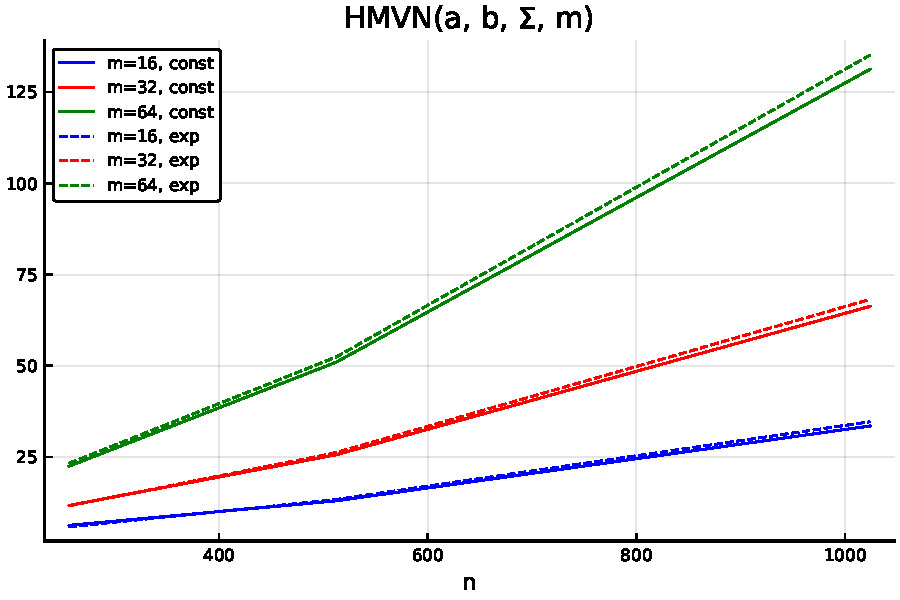
\includegraphics[width=0.8\linewidth]{figs/table3_m1.pdf}
		\caption{Execution time (seconds) for the hierarchical-block approximation}\label{fig:table3_htime}
	\end{figure}

	\framebreak

	\begin{figure}
		\centering
				\begin{subfigure}[b]{0.45\textwidth}
						\centering
						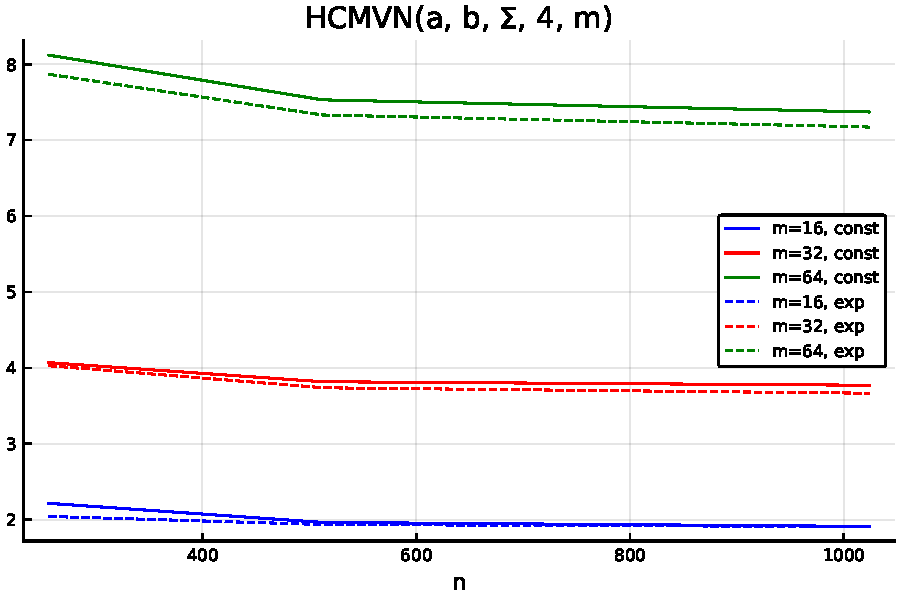
\includegraphics[width=\linewidth]{figs/table3_m2.pdf}
						\caption{\texttt{HCMVN}}
				\end{subfigure}\hfill
				\begin{subfigure}[b]{0.45\textwidth}
						\centering
						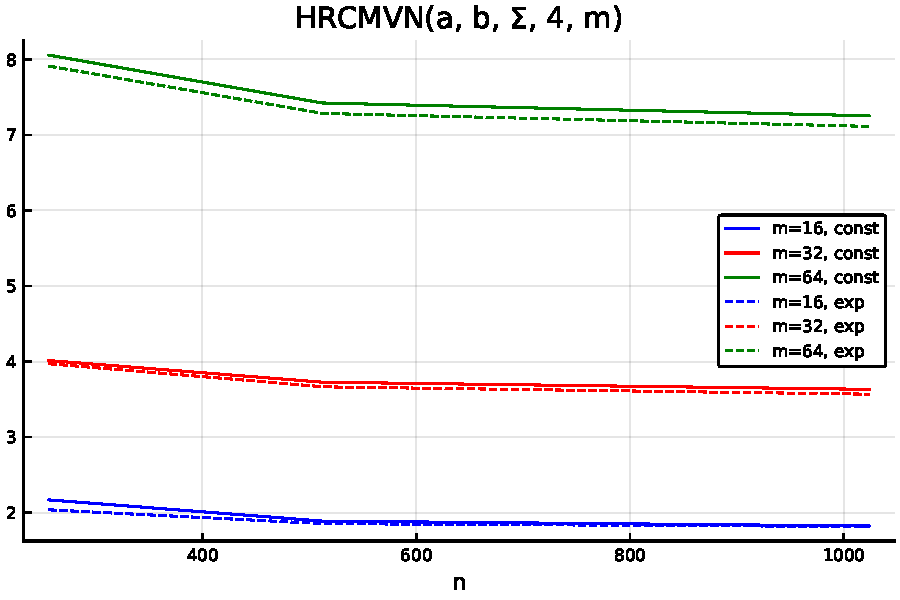
\includegraphics[width=\linewidth]{figs/table3_m3.pdf}
						\caption{\texttt{HRCMVN}}
				\end{subfigure}
		\caption{Execution time (seconds) for the hierarchical-block conditioning approximation}\label{fig:table3_hctime}
	\end{figure}	

	% The excution times of \texttt{HCMVN} and \texttt{HRCMVN} are significantly smaller than of \texttt{HMVN} even their performances are similar 

\end{frame}